\documentclass[11pt]{article}
\usepackage[T1]{fontenc}
\usepackage{lmodern}
\usepackage[margin=1in]{geometry}
\usepackage{microtype,amsmath,amssymb,graphicx,booktabs,array,placeins,float}
\usepackage{xcolor}
\usepackage[colorlinks=true,linkcolor=blue!50!black,citecolor=blue!50!black,urlcolor=blue!50!black]{hyperref}
\hypersetup{pdftitle={When AI Advisors Agree: Distinguishing Forecast Risk from Forecast Reliability},pdfauthor={Russlan Ramdowar}}
\setlength{\parskip}{4pt}
\setlength{\parindent}{1em}
\setlength{\emergencystretch}{2em}
\renewcommand{\arraystretch}{1.15}
\renewcommand{\topfraction}{0.9}
\renewcommand{\textfraction}{0.07}
\renewcommand{\floatpagefraction}{0.85}
\newcommand{\pp}{\text{pp}}
\title{When AI Advisors Agree:\\Distinguishing Forecast Risk from Forecast Reliability}
\author{Russlan Ramdowar\\\small Future Edge Group FZE, United Arab Emirates\\\small iPulse AI\\\small\texttt{russlan@ipulseai.com}\\\small ORCID: \href{https://orcid.org/0009-0004-9311-6957}{0009-0004-9311-6957}}
\date{9 October 2026}
\begin{document}
\maketitle
\begin{abstract}
If seven AI advisors give similar forecasts, should we trust them more? Agreement can indicate useful shared evidence, but it can also reflect an asset that was easier to forecast in the first place. We examine this distinction using 928 completed first-quarter forecasts for 232 assets across four production batches of iPulse AI. Ten historical Gemini configurations are grouped into seven investment frameworks; their archived forecasts are compared with later market outcomes, without generating new reports. Mean absolute return error rises from 10.31 percentage points in the lowest-disagreement quartile to 21.05 in the highest. Yet a forecast of no price change shows almost the same increase, from 9.89 to 21.15. The relationship between disagreement and additional forecast error is not resolved after accounting for visible asset risk. Retaining the quarter of forecasts with lowest historical volatility produces lower error than retaining those with least disagreement: 7.97 versus 10.31 percentage points. Agreement about direction behaves differently. When at least six of seven frameworks share a direction, directional accuracy is higher, but return-magnitude error is also larger. These results distinguish three questions often collapsed into one confidence score: how risky the asset is, whether advisors agree on its direction, and how precisely they forecast its return. For this historical council, agreement is informative in specific ways; it is not a general certificate of forecast reliability.
\end{abstract}

\section{Introduction}
An AI council can produce a persuasive form of evidence: several advisors, different reasoning frameworks, and a common conclusion. Agreement is visible immediately; correctness arrives later. This gap makes consensus attractive as a confidence signal, especially in forecasting tasks where the answer does not yet exist. It also makes agreement easy to overinterpret.

Consider two assets. One has a stable price history, and seven advisors predict modest returns close to one another. The other is volatile, and their predictions differ widely. If the first council later has smaller errors, agreement appears to predict reliability. But a forecast that ignores the council and simply predicts no price change might have smaller errors on the first asset too. The council could be identifying \emph{forecast difficulty}, rather than identifying when its own judgment adds value.

This paper tests that distinction in the ordinary production archive of iPulse AI, an Open Agentic Investment Research Platform. Its research pipeline generates reports through configured investment frameworks and modes, followed by a synthesis layer. The present study isolates a transparent, equally weighted council from historical individual forecasts. It does not evaluate the evidence-weighted synthesizer, rank current provider models, or measure the profitability of an investment strategy. A separate study of this platform examines how model disclosure affects synthesis weights \cite{ramdowar2026}; here the question concerns subsequent realized outcomes.

We analyze four batches issued between April and July 2026. The central comparison asks whether forecast dispersion predicts error \emph{beyond} what is already visible in an asset's price variability and in a no-change baseline. We then distinguish agreement about numerical returns from agreement about up, flat, or down. These are related signals, but they answer different questions.

The contribution is an auditable outcome study with three connected results. First, a strong raw relationship between council disagreement and return error is largely mirrored by a simple baseline. Second, selecting forecasts by historical volatility performs better than selecting them by raw disagreement in this sample. Third, directional agreement has a positive association with directional accuracy while failing to identify more precise return estimates. Together, these findings show why a single agreement score can hide materially different notions of reliability.

\section{Related work}
The distinction between disagreement and uncertainty predates language models. Lahiri and Sheng \cite{lahiri2010} show, under their forecasting model, that dispersion among forecasters does not capture all uncertainty associated with future common shocks. Glas \cite{glas2020} documents that the disagreement--uncertainty relationship depends on the forecast setting and how the quantities are measured. Our study brings this concern into an operational AI council: a forecast-spread signal should be tested against ordinary, observable task risk before it is interpreted as model-specific confidence.

In machine learning, deep ensembles offer a practical route to uncertainty estimation \cite{lakshminarayanan2017}. Those results do not establish that prompt frameworks sharing a model backbone behave like independently trained ensemble members. For language models, Xiao et al.\ \cite{xiao2025} formalize and test relationships between generation consistency and correctness across several tasks. Their work motivates examining consistency empirically rather than assuming that it is a universal confidence measure. Our task differs in an important respect: answers are later market returns, rather than labels already available when generations are evaluated.

ForecastBench \cite{karger2024} emphasizes forecasts about genuinely future events. We likewise preserve the distinction between the generation date and the outcome date, but use archived production returns rather than a purpose-built question benchmark. This observational setting provides breadth at the cost of weaker control over the information supplied to each historical run.

Selective prediction studies the tradeoff between retaining more predictions and accepting more error \cite{elyaniv2010}. We use retention curves descriptively: how much error remains when a rule keeps only a specified fraction of forecasts? We do not transfer selective-classification guarantees to market returns. Finally, point-forecast evaluation requires attention to the forecast functional and scoring rule \cite{gneiting2011}. Our arithmetic council mean is evaluated under absolute error as a practical decision loss; it is not asserted to be an optimal conditional median. A median-aggregation sensitivity check addresses this choice.

\section{Study setting and cohort}
\subsection{A fixed historical council}
The frozen evaluation archive has an outcome cutoff of 8 October 2026. We use native first-quarter forecasts from Batches 3--6, rather than daily refreshes, partially completed paths, or longer horizons. Batch 7, issued in September, is excluded because its native first-quarter targets had not matured at the cutoff. Earlier batches are excluded from the primary panel because their coverage and horizon representations are not comparable to the selected four-batch council.

The eligible set contains ten configurations representing seven frameworks (Table~\ref{tab:frameworks}). These are platform persona labels for configured AI research perspectives, not forecasts made or endorsed by the named individuals. Four frameworks have a researcher mode; the other three have researcher and thinker modes. We first average modes within each framework, then average the seven framework forecasts. This gives each framework equal weight and prevents those with two modes from receiving twice the influence.

\begin{table}[htbp]
\centering\small
\begin{tabular}{llr}
\toprule
Framework label & Historical modes retained & Configurations\\
\midrule
Elon Musk & Researcher & 1\\
Michael Burry & Researcher & 1\\
Niccolo Machiavelli & Researcher & 1\\
Sherlock Holmes & Researcher & 1\\
Ray Dalio & Researcher; thinker & 2\\
Superintelligence & Researcher; thinker & 2\\
Warren Buffett & Researcher; thinker & 2\\
\midrule
Total & Seven framework perspectives & 10\\
\bottomrule
\end{tabular}
\caption{Fixed historical council. All configurations use archived Gemini model versions. Framework diversity is not provider diversity or statistical independence.}
\label{tab:frameworks}
\end{table}

The model-version identifiers change between the earlier and later pairs of batches; they are recorded in the companion data. Thus, ``fixed council'' means a fixed set of framework--mode configurations, not a constant model binary. Provider, prompt, and model-version effects are not separately identified. This study should not be read as a benchmark of the newest models or of all multi-agent architectures.

Of 1,242 candidate asset--batch date groups, 15 lack the complete ten-configuration set. The remaining 1,227 matched outcomes cover 376 assets. Requiring an asset in all four batches yields 233 assets and 932 outcomes. One asset lacks valid historical-risk coverage across all four batches, leaving the primary balanced panel of \textbf{232 assets and 928 outcomes}. The panel includes 206 equities, 14 crypto assets, five commodities, five foreign-exchange assets, and two funds. Each contributes four outcomes. Selection is based on completeness, not observed forecast accuracy, but requiring future coverage still introduces a retrospective survivorship constraint.

\begin{figure}[H]
\centering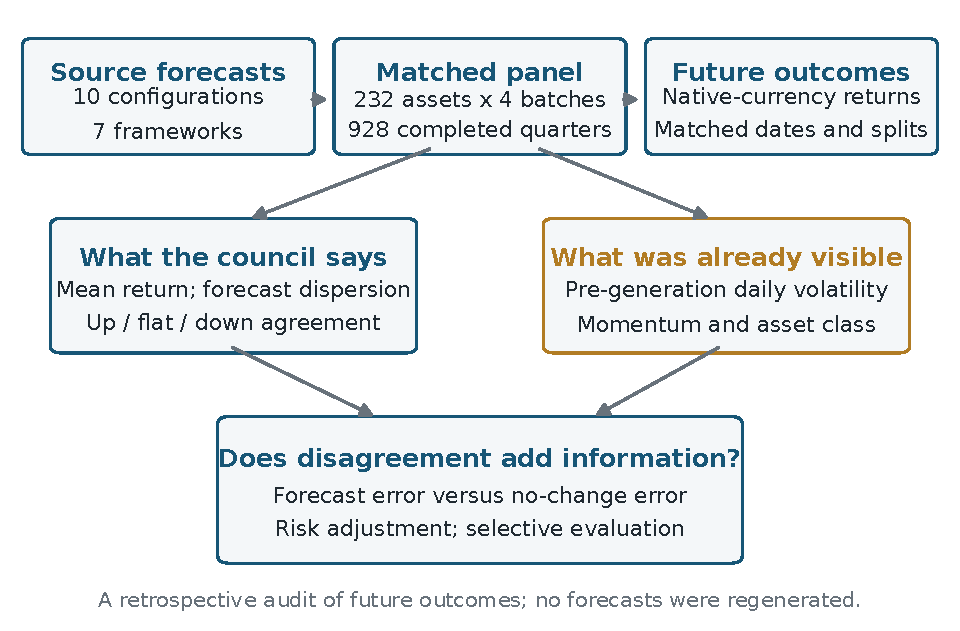
\includegraphics[width=\linewidth]{figures/01_study_design.pdf}
\caption{Study design. Seven framework-level forecasts are compared with later outcomes and with risk measures available from prices dated before generation. The analysis distinguishes raw error, error relative to a baseline, and selective evaluation.}
\label{fig:design}
\end{figure}

\subsection{The information clock matters}
Figure~\ref{fig:timing} shows the forecast and outcome windows. Much of Batch 3 had not matured when Batch 6 was generated, and the following batches had still less completed history available. Within the primary panel, only one earlier first-quarter outcome had closed before the Batch 6 issue date; none had closed before the Batch 4 or Batch 5 issue dates. Fitting an error predictor to all four batches and presenting it as a policy that could have been trained at each issuance would therefore be misleading.

Our retention rules require no fitted outcome labels. They rank assets within a batch using council dispersion, historical volatility, or their ratio. The later regression is explicitly a \emph{retrospective association analysis}, not a prospectively trained confidence model. Rules, cutoffs, and analyses were developed after an initial exploratory inspection; this study was not preregistered.

Forecast evaluation starts at the archive's first saved close after generation, rather than an assumed executable price at the exact generation time. Predicted target values and realized target prices are expressed relative to that common entry close. Consequently, these rebased scores become available at the entry close, not necessarily at the generation instant. The price-history risk measures use dates strictly before generation. This construction aligns forecasts with a common evaluable return, without implying that a live trade was placed.

\begin{figure}[htbp]
\centering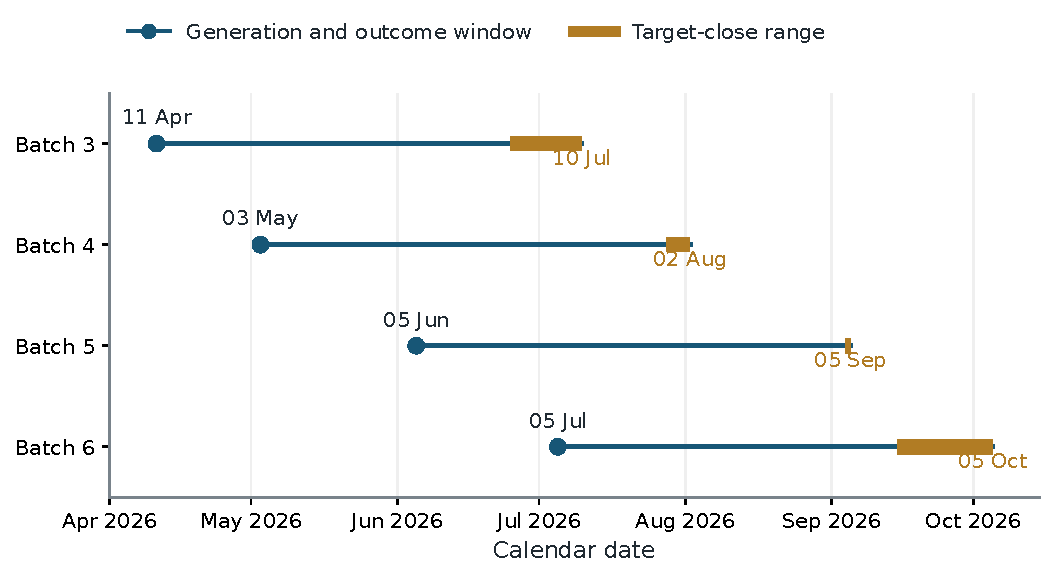
\includegraphics[width=\linewidth]{figures/02_timing.pdf}
\caption{Overlapping first-quarter outcome windows. Blue circles mark generation dates; gold segments mark the range of target-close observations across assets. Most preceding-quarter labels were unavailable at the next generation. The figure explains why adjusted models are treated as retrospective diagnostics.}
\label{fig:timing}
\end{figure}
\FloatBarrier

\section{Measures and analysis}
\subsection{Agreement, error, and the baseline}
For asset $a$ in batch $b$, let $p_{abj}$ be the predicted percentage return of framework $j$, after averaging its retained modes, and let $y_{ab}$ be the realized percentage return. With $J=7$, the council return and numerical disagreement are
\begin{equation}
\bar p_{ab}=\frac{1}{J}\sum_{j=1}^{J}p_{abj},\qquad
D_{ab}=\sqrt{\frac{1}{J}\sum_{j=1}^{J}(p_{abj}-\bar p_{ab})^2}.
\end{equation}
The population standard deviation describes the spread of this specified council. It is not a predictive standard error, an estimate based on seven independent draws, or a probability interval for the future return.

Absolute return error, no-change error, and their difference are
\begin{equation}
E_{ab}=|\bar p_{ab}-y_{ab}|,\qquad E^0_{ab}=|y_{ab}|,\qquad
\Delta E_{ab}=E_{ab}-E^0_{ab}.
\end{equation}
All are measured in percentage points (pp). Positive $\Delta E$ means the council does worse than predicting a zero return; negative values mean it does better. Subtracting this simple baseline does not remove every source of forecast difficulty. It does show whether a raw error pattern also occurs without using the advisors' predicted return.

Directional agreement is measured separately. A return above $+0.5$ pp is up, below $-0.5$ pp is down, and otherwise flat. Let $s(p)$ denote this classification. Then
\begin{equation}
A_{ab}=\max_{c\in\{-1,0,1\}}\frac{1}{J}\sum_{j=1}^{J}\mathbf{1}\{s(p_{abj})=c\}.
\end{equation}
High directional agreement means $A\geq6/7$. Directional accuracy evaluates the sign of the \emph{council mean}, not the modal framework sign. An extreme forecast can therefore make the two disagree. We compare directional accuracy with an always-up baseline; predicting no change is the appropriate separate baseline for return error.

\subsection{Visible asset risk}
Historical volatility is computed from the most recent 60 observed daily log returns before generation, requiring at least 45 observations. Recorded active splits are incorporated into the historical returns. A conservative check excludes histories with an unsupported large split adjustment; 20- and 90-observation windows provide sensitivity comparisons.

To place volatility on the approximate horizon scale, define
\begin{equation}
V_{ab}=100\,\hat\sigma_{ab}\sqrt{h_{ab}\,n_a/365},
\end{equation}
where $h$ is the number of calendar days from entry to target, and $n_a$ is 365 for crypto assets and 252 otherwise. This square-root scaling is a conventional descriptive risk measure, not a claim that returns are Gaussian or independent. Historical momentum is the cumulative return over the same 60-observation window. All outcomes are native-currency price returns; they do not include dividend reinvestment or a common-currency portfolio conversion.

\subsection{Comparisons and uncertainty}
We assign disagreement quartiles \emph{within each batch}, so a change in the overall forecast scale cannot alone create the pooled gradient. Each primary quartile contains 58 assets per batch, or 232 outcomes. We also form five within-batch volatility groups and compare lower and higher disagreement within each group.

The adjusted model relates $\log(1+E)$ to historical volatility, absolute forecast magnitude, absolute historical momentum, and disagreement, with batch and asset-class indicators. Continuous predictors are transformed and standardized; exact definitions appear in Appendix~\ref{app:reproduce}. A second model uses $\Delta E$ as the response. These controls test conditional associations in this sample. They do not identify a causal effect of disagreement, remove all risk, or establish the absence of a small useful signal.

For selective evaluation, we retain the lowest 25\%, 50\%, 75\%, or 100\% of scores within each batch and measure subsequent error among those retained. The selectors are $D$, $V$, and $D/V$. These are descriptive coverage comparisons, not an investment backtest: they contain no position sizing, execution, transaction costs, or utility objective.

We report pointwise 95\% percentile intervals from 5,000 asset-cluster bootstrap draws, resampling entire assets with their four outcomes together. Regression intervals use 2,000 draws. Paired contrasts use the same cluster draws for both groups or selectors. Intervals condition on the archived observations and fixed rank membership. They account for repeated assets, but not fully for common market shocks across assets or the four overlapping periods. They are neither simultaneous intervals nor prospective performance guarantees.

\section{Results}
\subsection{The apparent confidence signal mirrors a simple baseline}
Numerical disagreement strongly separates later absolute error. Mean error rises from 10.31 pp in the lowest-disagreement quartile to 21.05 pp in the highest (Figure~\ref{fig:quartiles}). The high-minus-low gap is 10.74 pp, with a 95\% interval of [7.11, 14.78]. Viewed alone, this looks like a useful confidence signal.

The no-change baseline, however, rises almost identically: 9.89 pp to 21.15 pp. Its high-minus-low gap is 11.26 pp [7.82, 15.10]. The corresponding gap in error \emph{beyond the baseline} is $-0.52$ pp [$-1.74$, 0.69]. Thus, the raw gradient does not establish that low disagreement identifies greater council skill. Much of the separation also describes how far prices subsequently move from their starting values.

\begin{table}[htbp]
\centering\small
\begin{tabular}{lrrrr}
\toprule
Disagreement quartile & Council MAE & No-change MAE & Difference & Mean $V$\\
\midrule
Lowest & 10.31 & 9.89 & +0.41 & 14.31\\
Second & 13.14 & 13.09 & +0.05 & 16.91\\
Third & 16.10 & 15.81 & +0.29 & 21.21\\
Highest & 21.05 & 21.15 & $-0.10$ & 30.03\\
\bottomrule
\end{tabular}
\caption{Within-batch disagreement quartiles, pooled across four batches; 232 outcomes per row. Return errors and horizon-scaled volatility $V$ are in pp. Rounded entries may not subtract exactly.}
\label{tab:quartiles}
\end{table}

\begin{figure}[htbp]
\centering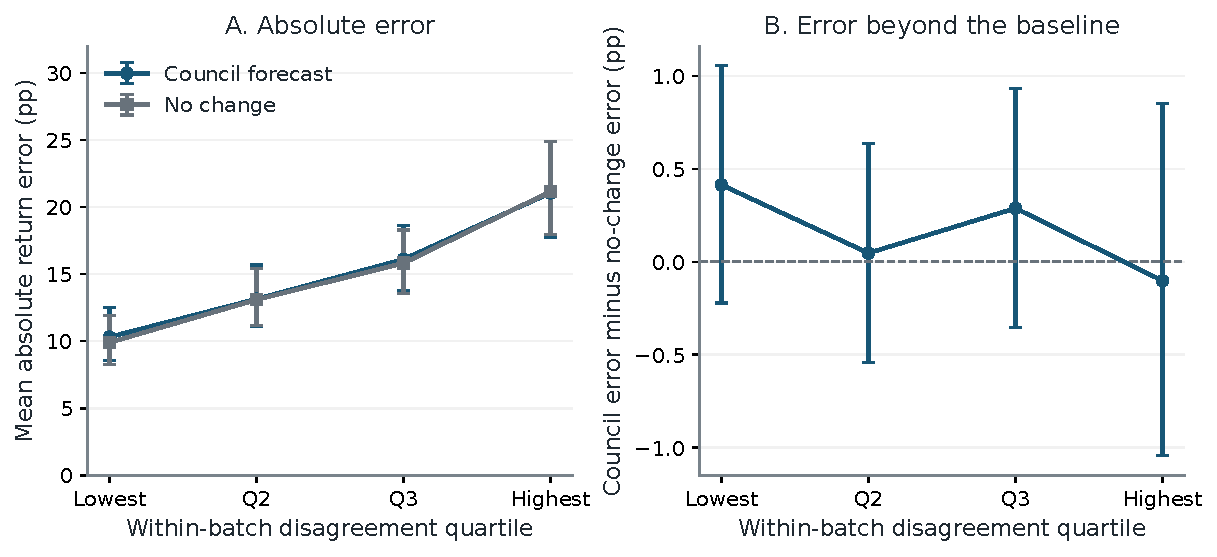
\includegraphics[width=\linewidth]{figures/03_disagreement_and_baseline.pdf}
\caption{The raw disagreement--error gradient is also present for no change. A: absolute errors for the council and baseline. B: their paired difference within each quartile. Bars are pointwise asset-cluster 95\% intervals.}
\label{fig:quartiles}
\end{figure}

Across the full panel, council MAE is 15.15 pp versus 14.99 pp for no change. The paired difference is +0.16 pp [$-0.23$, 0.56]. Council directional accuracy is 48.38\%, compared with 50.75\% for always up. These aggregate comparisons provide no clear evidence of an overall advantage under the chosen losses. They do not prove that the systems are equivalent, nor do they evaluate the quality of their qualitative research.

\subsection{Disagreement tracks risk visible before generation}
The raw gradient has a plausible, observable explanation. Disagreement and historical volatility have within-batch Spearman correlations between 0.56 and 0.69 (Figure~\ref{fig:risk}). Historical volatility also correlates with subsequent council error, more strongly than disagreement does in each of the four batches. Advisors tend to spread their forecasts more widely on assets whose recent price behavior already signals greater variability.

\begin{figure}[htbp]
\centering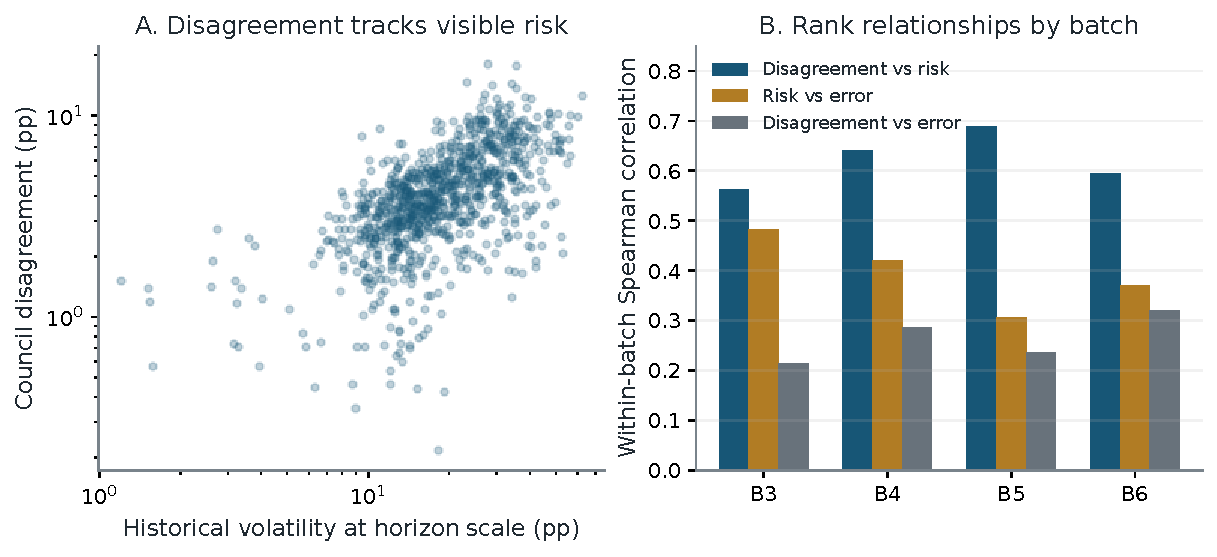
\includegraphics[width=\linewidth]{figures/04_visible_risk.pdf}
\caption{Visible asset risk and council dispersion. A: 928 outcomes plotted on logarithmic axes. B: within-batch rank correlations. The council's spread is closely related to historical volatility, which is more strongly related to absolute forecast error than spread is in each batch.}
\label{fig:risk}
\end{figure}

In the adjusted model, the standardized log-disagreement coefficient for $\log(1+E)$ is 0.006 [$-0.072$, 0.079], while the historical-volatility coefficient is 0.358 [0.259, 0.465]. The disagreement coefficient in the excess-error model is $-0.08$ pp [$-0.63$, 0.42]. These estimates do not resolve an additional association after the specified controls; they are not an equivalence test.

The coarse, less model-dependent comparison gives a similar result. Within volatility groups, higher-disagreement forecasts have a mean error 1.02 pp lower than lower-disagreement forecasts, with an interval spanning both directions [$-3.99$, 1.79]. Their excess-error difference is $-0.31$ pp [$-1.04$, 0.41]. A strong unconditional association is therefore insufficient to justify treating dispersion as a distinct reliability measure.

\begin{figure}[htbp]
\centering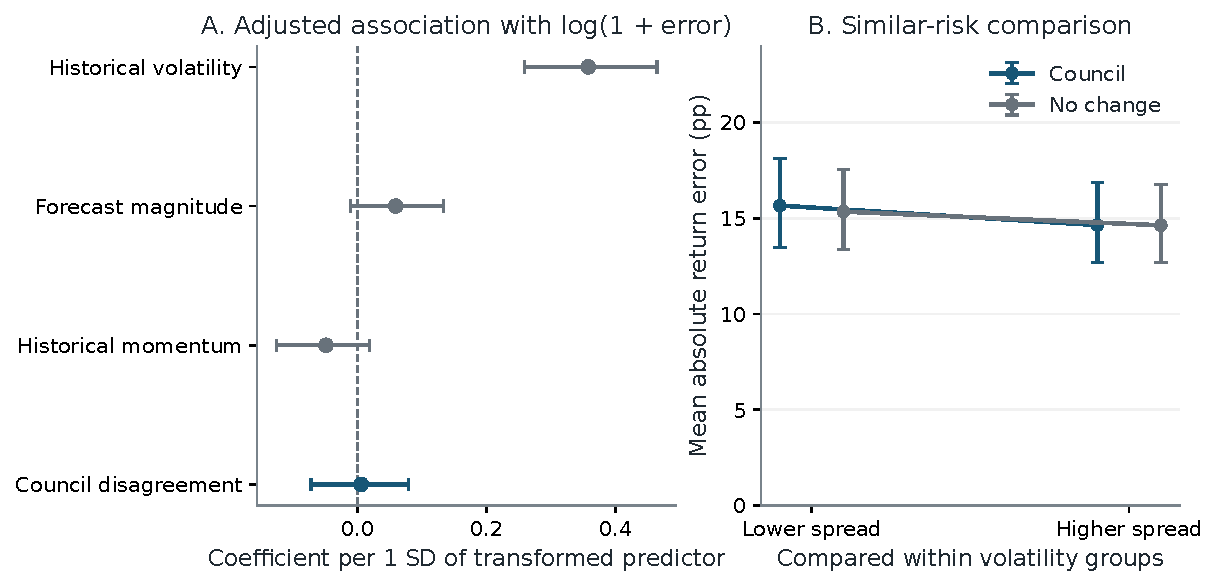
\includegraphics[width=\linewidth]{figures/06_adjusted_comparison.pdf}
\caption{Adjusted and similar-risk comparisons. A: coefficients for standardized transformed predictors in the model of $\log(1+E)$, controlling for batch and asset class. B: lower and higher disagreement within five volatility groups per batch. Bars show pointwise asset-cluster 95\% intervals. These are retrospective diagnostics.}
\label{fig:adjusted}
\end{figure}
\FloatBarrier

\subsection{A cheaper observable ranks low-error forecasts better}
Selecting the least-disagreeing quarter of forecasts reduces MAE from 15.15 pp to 10.31 pp. Selecting the lowest-volatility quarter reduces it further, to 7.97 pp (Figure~\ref{fig:coverage}). The paired difference between the volatility and disagreement selectors is $-2.34$ pp [$-4.26$, $-0.80$]. Both rules retain 58 assets per batch, but need not retain the same assets.

This improvement is about selecting easier cases, not demonstrating greater forecasting skill. On the lowest-volatility quarter, no change has MAE 8.00 pp; the council-minus-baseline difference is $-0.03$ pp [$-0.43$, 0.37]. On the least-disagreeing quarter, the council's difference is +0.41 pp. A selection rule can substantially reduce error while leaving the council's advantage over the baseline unresolved.

Dividing disagreement by volatility does not automatically produce a better confidence signal. Keeping the lowest $D/V$ quarter yields MAE 18.45 pp. A large denominator can make a volatile asset appear to have small relative disagreement. This failed shortcut is useful: controlling for risk in an analysis and constructing a reliable selection score are different tasks.

\begin{figure}[htbp]
\centering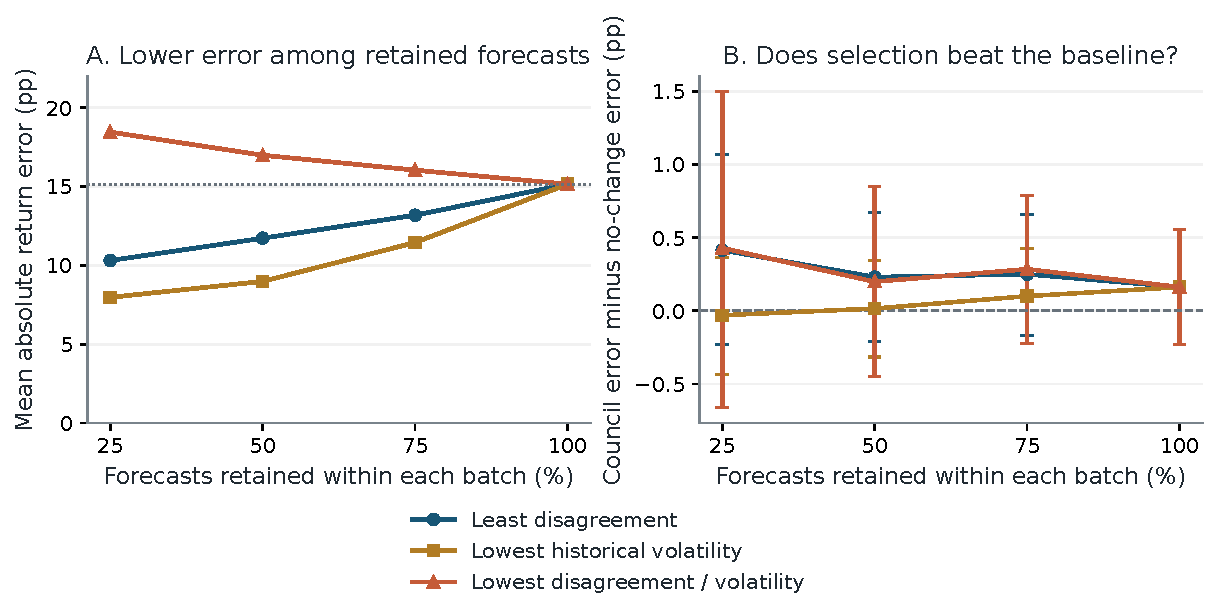
\includegraphics[width=\linewidth]{figures/05_selective_evaluation.pdf}
\caption{Selective evaluation at equal within-batch coverage. A: absolute error among retained forecasts. B: paired error relative to no change, with pointwise cluster intervals. At 100\% all rules retain the same panel. The rules require no fitted outcome labels; their evaluation is retrospective.}
\label{fig:coverage}
\end{figure}

\subsection{Agreement about direction is a different signal}
High directional agreement occurs in 436 outcomes; the other 492 have fewer than six frameworks sharing a direction. Council directional accuracy is 53.21\% in the high-agreement group versus 44.11\% in the other group (Figure~\ref{fig:direction}). The difference is 9.11 percentage points [3.03, 15.22]. The corresponding contrast in accuracy relative to always up is 11.39 points [1.95, 20.96]. The descriptive association is therefore not explained simply by there being more upward outcomes in the high-agreement group.

Return precision moves in the opposite direction. The high-agreement group has MAE 16.84 pp, compared with 13.65 pp in the other group: a difference of +3.19 pp [0.73, 5.80]. Six advisors can agree that a price will rise while disagreeing substantially about how much, or while jointly misjudging its magnitude. Numerical dispersion and directional concordance should not be used interchangeably.

This is a secondary, exploratory finding under an explicit threshold. The unadjusted association may reflect asset composition and trend conditions. It supports further testing of direction-specific confidence, not a claim that 53.21\% is a calibrated probability or that the rule is profitable. It has not been validated on an untouched subsequent batch.

\begin{figure}[htbp]
\centering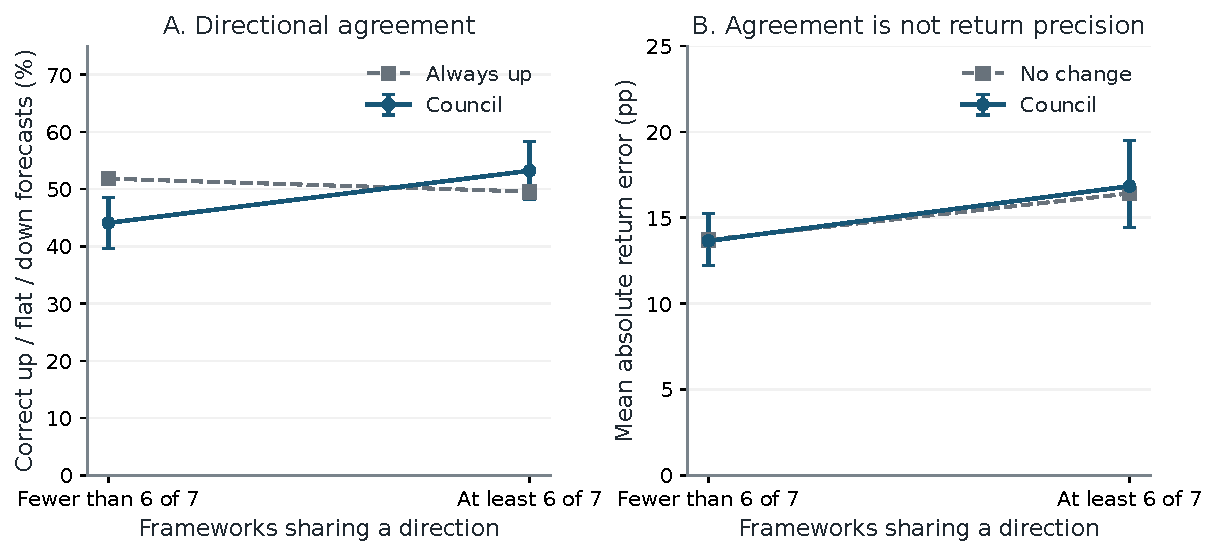
\includegraphics[width=\linewidth]{figures/07_direction_vs_magnitude.pdf}
\caption{Directional concordance does not imply numerical precision. A: council directional accuracy and the always-up baseline. B: return MAE and no-change MAE for the same groups. Council error bars are pointwise asset-cluster 95\% intervals; baseline markers show estimates.}
\label{fig:direction}
\end{figure}

\FloatBarrier
\subsection{Robustness and variation across batches}
The central excess-error contrast remains unresolved when we expand coverage to 1,221 outcomes, restrict to equities, require original published-cohort membership, remove the largest 1\% of errors, replace the council mean with its median, or score against the original forecast anchor (Figure~\ref{fig:robustness}). Every corresponding interval spans zero. Alternative spread measures also give unresolved high-minus-low excess-error gaps: +0.11 pp [$-0.92$, 1.17] for the interquartile range and $-0.42$ pp [$-1.46$, 0.61] for median absolute deviation.

The lowest-volatility quarter remains a low-error subset with 20- and 90-observation windows: MAE is 7.60 and 7.50 pp, respectively. Their council-minus-no-change differences are small, with intervals spanning zero. Root mean squared errors rise across disagreement quartiles for both the council and baseline as well (Appendix~\ref{app:tables}). Thus, the visible raw gradient is not peculiar to a single absolute-error calculation.

The pooled council--baseline comparison also varies by batch. Batch 3 has council MAE 18.88 pp versus 16.97 pp for no change; the other three batches have small mean advantages for the council (Table~\ref{tab:batches}). This variation cautions against interpreting the pooled near-zero difference as a stable characteristic of the platform. The available record contains only four overlapping evaluation periods.

\begin{figure}[htbp]
\centering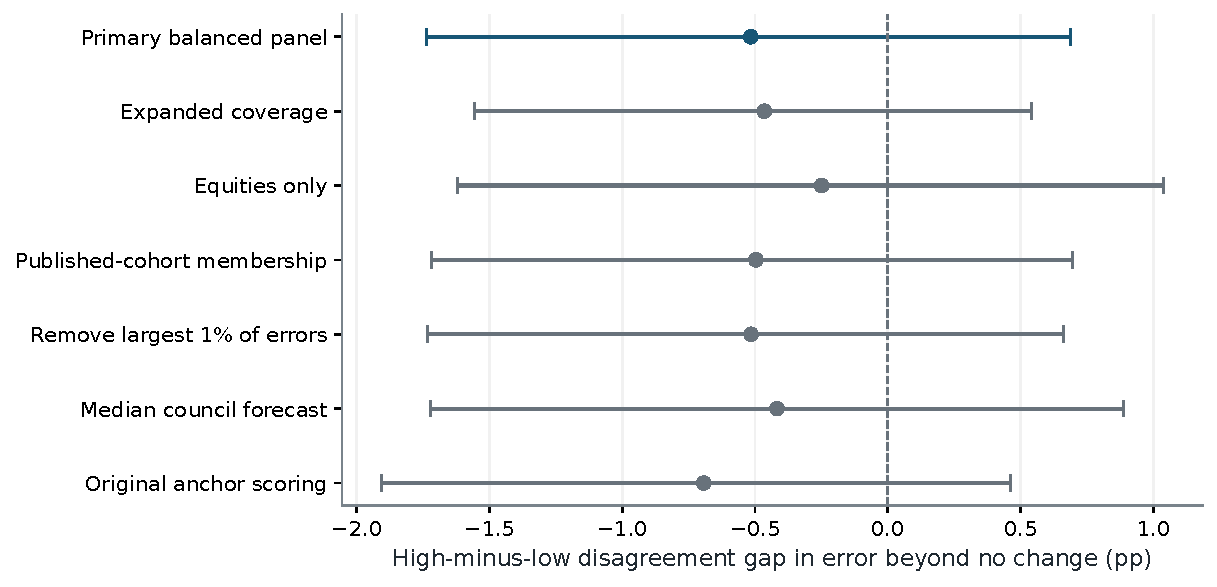
\includegraphics[width=\linewidth]{figures/08_robustness.pdf}
\caption{Sensitivity of the high-minus-low disagreement contrast in excess error. Negative values indicate a smaller council-minus-baseline error in the highest-disagreement quartile. Pointwise asset-cluster 95\% intervals span zero across the listed specifications.}
\label{fig:robustness}
\end{figure}
\FloatBarrier

\section{What an agreement score should communicate}
The results suggest separating three concepts in an AI forecasting system. \emph{Asset risk} concerns how variable the outcome may be. \emph{Directional concordance} concerns whether the advisors share an up, flat, or down view. \emph{Return precision} concerns how close their numerical prediction is to the eventual return. A score that blends these concepts can appear predictive while obscuring what it actually predicts.

For this council, historical volatility is a strong first reference for forecast difficulty. Council dispersion adds no clearly resolved relationship with excess error under the tested comparisons. Directional agreement, however, has a positive association with directional accuracy. The conclusion is therefore more specific than ``agreement is useless'': different forms of agreement carry different information, and none should be advertised as universal confidence without further validation.

A sensible next test would freeze the feature definitions and thresholds before a new batch, register the available training labels, and evaluate direction and return losses separately after the native targets mature. If an error predictor is learned, validation must respect both the issue date and the maturity date of every label. A model trained on future-resolved labels cannot be presented as a real-time confidence layer merely because the forecasts themselves were made earlier.

This archive does not contain the consistent predictive distributions needed to establish probabilistic calibration. A seven-framework spread cannot be labeled an 80\% or 95\% confidence interval without an additional, validated mapping to outcome coverage. Similarly, being more accurate on a retained subset does not establish an economic advantage. Such claims require a defined decision rule and appropriate costs, baselines, and out-of-time testing.

\section{Limitations}
\paragraph{One system and few periods.} The council shares historical Gemini model versions, and the four forecast periods overlap. Framework diversity is neither independence nor diversity across providers. Asset-cluster intervals preserve repeated assets but cannot eliminate dependence induced by common market shocks. Generalization to other models, markets, horizons, or regimes remains untested.

\paragraph{Retrospective coverage and data vintage.} Assets were curated for a production platform and then required to have complete forecasts and history. They are not a random sample of the investable universe. The evaluation uses a frozen October archive, not an immutable contemporaneous market-data vintage for every past day. Revised prices, corporate actions, and reconstructed context can differ from what was available during the original run. The analysis respects dates in the archive but cannot independently certify the full historical information set of every prompt.

\paragraph{Scoring and operational choices.} Native-currency price returns exclude dividend reinvestment, currency conversion, and execution costs. Evaluation is rebased to a saved post-generation close, rather than an assumed trade at the generation instant. The council mean, volatility scaling, sign threshold, and retention fractions are choices; the reported sensitivities address some, not all, alternatives. Qualitative report quality and synthesized portfolio recommendations are outside the scope.

\paragraph{Exploration and unresolved effects.} The analyses follow an exploratory audit rather than a preregistration. Multiple secondary comparisons are not multiplicity-adjusted. Intervals overlapping zero do not demonstrate equivalence or rule out small useful effects. In particular, the directional-agreement result merits prospective confirmation before it is used as a confidence rule.

\section{Conclusion}
In this historical AI council, wider numerical disagreement predicts larger return errors, but nearly the same pattern occurs for a no-change forecast and is strongly associated with visible asset volatility. A simple volatility rule selects lower-error forecasts more effectively than raw disagreement. Agreement about direction has a different association: better directional accuracy, accompanied by larger numerical errors. The practical lesson is to evaluate agreement against the question it is meant to answer. Before calling consensus a confidence signal, establish whether it measures ordinary outcome risk, shared directional judgment, or an actual improvement in forecast reliability.

\section*{Data, code, and author disclosure}
The \href{https://doi.org/10.5281/zenodo.23262216}{Zenodo research deposit} (DOI: \href{https://doi.org/10.5281/zenodo.23262216}{10.5281/zenodo.23262216}) and \href{https://github.com/TheFutureEdge/research-when-ai-advisors-agree}{public research repository} contain individual configuration forecasts, cohort metadata, aggregate results, deterministic analysis code, and vector figures. The frozen source-archive fingerprint and extraction rules are documented. The full market-derived outcome panel, raw market-history files, credentials, and operational metadata are excluded from the public release. Recomputing outcome-dependent results requires compatible market inputs obtained under appropriate terms or authorized access to the author-side panel. Historical values come from the iPulse AI market-history archive; no alternative source attribution is implied. Original manuscript, figures, forecast data, and research summaries use CC BY 4.0; code uses MIT. Third-party material retains its applicable terms.

The author is the founder of Future Edge Group FZE, which develops iPulse AI, and has a commercial interest in the platform studied. AI systems assisted with research operations, coding, audit, and manuscript preparation. Authorship and responsibility for the final submission remain with the named human author.

\begin{thebibliography}{9}
\bibitem{lahiri2010} K. Lahiri and X. Sheng. Measuring forecast uncertainty by disagreement: The missing link. \emph{Journal of Applied Econometrics}, 25:514--538, 2010. \href{https://doi.org/10.1002/jae.1167}{doi:10.1002/jae.1167}.
\bibitem{glas2020} A. Glas. Five dimensions of the uncertainty--disagreement linkage. \emph{International Journal of Forecasting}, 36(2):607--627, 2020. \href{https://doi.org/10.1016/j.ijforecast.2019.07.010}{doi:10.1016/j.ijforecast.2019.07.010}.
\bibitem{lakshminarayanan2017} B. Lakshminarayanan, A. Pritzel, and C. Blundell. Simple and scalable predictive uncertainty estimation using deep ensembles. \emph{Advances in Neural Information Processing Systems}, 30, 2017. \href{https://proceedings.neurips.cc/paper/2017/hash/9ef2ed4b7fd2c810847ffa5fa85bce38-Abstract.html}{NeurIPS proceedings}.
\bibitem{xiao2025} Q. Xiao, D. Bhattacharjya, B. Ganesan, R. Marinescu, K. Mirylenka, N. H. Pham, M. Glass, and J. Lee. The consistency hypothesis in uncertainty quantification for large language models. \emph{Proceedings of the Forty-first Conference on Uncertainty in Artificial Intelligence}, PMLR 286:4636--4651, 2025. \href{https://proceedings.mlr.press/v286/xiao25a.html}{PMLR proceedings}.
\bibitem{karger2024} E. Karger, H. Bastani, Chen Yueh-Han, Z. Jacobs, D. Halawi, F. Zhang, and P. E. Tetlock. ForecastBench: A dynamic benchmark of AI forecasting capabilities. \emph{arXiv:2409.19839}, 2024, revised 2025. \url{https://arxiv.org/abs/2409.19839}.
\bibitem{elyaniv2010} R. El-Yaniv and Y. Wiener. On the foundations of noise-free selective classification. \emph{Journal of Machine Learning Research}, 11:1605--1641, 2010. \href{https://www.jmlr.org/papers/v11/el-yaniv10a.html}{JMLR article}.
\bibitem{gneiting2011} T. Gneiting. Making and evaluating point forecasts. \emph{Journal of the American Statistical Association}, 106(494):746--762, 2011. \href{https://doi.org/10.1198/jasa.2011.r10138}{doi:10.1198/jasa.2011.r10138}.
\bibitem{ramdowar2026} R. Ramdowar. When models judge models: How source identity and disagreement shape multi-agent financial forecasts. iPulse AI research artifacts, 2026. \href{https://doi.org/10.5281/zenodo.23083356}{doi:10.5281/zenodo.23083356}.
\end{thebibliography}

\clearpage
\appendix
\section{Reproduction and cohort details}\label{app:reproduce}
The analysis cutoff is 8 October 2026; the manuscript date is 9 October. The input is identified by SHA-256\footnote{\texttt{f4f9510fe0ae2900f124b12e638f06eac073f0397c5646e6dfea62a278555be1}.}. Source extraction selects completed native first-quarter observations in Batches 3--6 with the eligible ten configurations. Matching requires one observation per configuration, identical entry and target dates, a common issue date, finite predictions, and realized returns agreeing to tolerance $10^{-6}$. No forecast is regenerated.

The expanded matched panel has 242, 307, 303, and 375 outcomes in Batches 3, 4, 5, and 6. The primary panel has 232 in each. The one balanced asset excluded for risk validity contributes four outcomes; its omission is not based on its forecast error. The author-side derived panel preserves exclusion flags and coverage variables for auditing; the public cohort file identifies matched records and primary membership.

Daily historical returns use positive finite closes before the issue date. Between consecutive observations, split ratios with recorded active ex-dates are applied. Histories are quarantined when a split adjustment produces an absolute daily log move above 0.4 while the unadjusted move is below 0.2. This heuristic conservatively avoids a possible double adjustment; it is not a general corporate-action validator. Momentum uses the last 60 available log returns. Historical volatility uses the sample standard deviation and at least 75\% of the requested observation window, with a minimum of 15 observations.

For the adjusted model, continuous variables are $\log V$, $\log(1+|\text{momentum}|)$, $\log(1+|\bar p|)$, and $\log(1+D)$. Each is standardized using the primary panel's mean and population standard deviation. Ordinary least squares includes batch and asset-class indicators; bootstrap refits preserve each asset's complete cluster. The random seed is 20261009. No fitted model is claimed to be deployable at historical issue dates.

A numerical tolerance of $10^{-10}$ pp at the $\pm0.5$ pp sign boundaries prevents floating-point classification artifacts.

For retained fractions, assets are sorted within each batch by score, breaking ties with the stable asset identifier; the retained count is rounded upward. The bootstrap holds this selection membership fixed. For the within-risk contrast, assets are sorted into five approximately equal-sized volatility bins per batch, then split into lower and higher disagreement halves within each bin. These finite-sample comparisons cannot eliminate all continuous-risk differences.

\section{Additional numerical results}\label{app:tables}
\begin{table}[htbp]
\centering\small
\begin{tabular}{lrrrrr}
\toprule
Batch & Council MAE & No-change MAE & Difference & Direction & Always up\\
\midrule
3 & 18.88 & 16.97 & +1.91 & 38.36\% & 52.16\%\\
4 & 13.70 & 14.21 & $-0.51$ & 50.43\% & 51.72\%\\
5 & 13.47 & 14.08 & $-0.62$ & 53.88\% & 59.91\%\\
6 & 14.54 & 14.68 & $-0.14$ & 50.86\% & 39.22\%\\
\bottomrule
\end{tabular}
\caption{Batch-level estimates in the primary panel, 232 outcomes per row. Return errors are in pp. Direction uses the three-category sign rule; always up is a separate directional baseline.}
\label{tab:batches}
\end{table}

\begin{table}[htbp]
\centering\small
\begin{tabular}{lrr}
\toprule
Disagreement quartile & Council RMSE (pp) & No-change RMSE (pp)\\
\midrule
Lowest & 17.69 & 16.55\\
Second & 21.01 & 20.07\\
Third & 23.39 & 22.79\\
Highest & 31.14 & 30.63\\
\bottomrule
\end{tabular}
\caption{Squared-error sensitivity. Both series exhibit increasing error across disagreement quartiles. This table supplies a second loss function, not a fitted probabilistic forecast evaluation.}
\end{table}

\begin{table}[htbp]
\centering\small
\begin{tabular}{lrrr}
\toprule
Volatility window & Retained outcomes & Council MAE (pp) & Excess MAE (pp)\\
\midrule
20 observations & 232 & 7.60 & +0.08 [$-0.31$, 0.45]\\
60 observations & 232 & 7.97 & $-0.03$ [$-0.43$, 0.37]\\
90 observations & 232 & 7.50 & +0.02 [$-0.36$, 0.41]\\
\bottomrule
\end{tabular}
\caption{Lowest-volatility quarter under alternative historical windows. Brackets are pointwise asset-cluster 95\% intervals for the paired error difference relative to no change.}
\end{table}

\FloatBarrier
The public CSVs permit checking forecast grouping and cohort membership. \texttt{prepare\_panel.py} documents extraction from the private frozen archive; \texttt{analyze.py} and \texttt{make\_figures.py} require the full derived author-side panel to recompute outcome-dependent tables and figures. That panel is retained privately, together with an executed notebook and independent validation checks. No production service calls or new model generations are required when compatible inputs are available. The public release therefore exposes the forecasts, methods, code, and aggregate findings, but is not a fully self-contained outcome-replication dataset. The arXiv source bundle contains only the manuscript, bibliography, and referenced figures.
\end{document}
